\documentclass[]{article}
\usepackage{lmodern}
\usepackage{amssymb,amsmath}
\usepackage{ifxetex,ifluatex}
\usepackage{fixltx2e} % provides \textsubscript
\ifnum 0\ifxetex 1\fi\ifluatex 1\fi=0 % if pdftex
  \usepackage[T1]{fontenc}
  \usepackage[utf8]{inputenc}
\else % if luatex or xelatex
  \ifxetex
    \usepackage{mathspec}
  \else
    \usepackage{fontspec}
  \fi
  \defaultfontfeatures{Ligatures=TeX,Scale=MatchLowercase}
\fi
% use upquote if available, for straight quotes in verbatim environments
\IfFileExists{upquote.sty}{\usepackage{upquote}}{}
% use microtype if available
\IfFileExists{microtype.sty}{%
\usepackage{microtype}
\UseMicrotypeSet[protrusion]{basicmath} % disable protrusion for tt fonts
}{}
\usepackage[margin=1in]{geometry}
\usepackage{hyperref}
\PassOptionsToPackage{usenames,dvipsnames}{color} % color is loaded by hyperref
\hypersetup{unicode=true,
            pdftitle={User Guide: Science-Wise False Discovery Rate},
            pdfauthor={Nathan (Nat) Goodman},
            colorlinks=true,
            linkcolor=cyan,
            citecolor=green,
            urlcolor=blue,
            breaklinks=true}
\urlstyle{same}  % don't use monospace font for urls
\usepackage{color}
\usepackage{fancyvrb}
\newcommand{\VerbBar}{|}
\newcommand{\VERB}{\Verb[commandchars=\\\{\}]}
\DefineVerbatimEnvironment{Highlighting}{Verbatim}{commandchars=\\\{\}}
% Add ',fontsize=\small' for more characters per line
\usepackage{framed}
\definecolor{shadecolor}{RGB}{248,248,248}
\newenvironment{Shaded}{\begin{snugshade}}{\end{snugshade}}
\newcommand{\KeywordTok}[1]{\textcolor[rgb]{0.13,0.29,0.53}{\textbf{{#1}}}}
\newcommand{\DataTypeTok}[1]{\textcolor[rgb]{0.13,0.29,0.53}{{#1}}}
\newcommand{\DecValTok}[1]{\textcolor[rgb]{0.00,0.00,0.81}{{#1}}}
\newcommand{\BaseNTok}[1]{\textcolor[rgb]{0.00,0.00,0.81}{{#1}}}
\newcommand{\FloatTok}[1]{\textcolor[rgb]{0.00,0.00,0.81}{{#1}}}
\newcommand{\ConstantTok}[1]{\textcolor[rgb]{0.00,0.00,0.00}{{#1}}}
\newcommand{\CharTok}[1]{\textcolor[rgb]{0.31,0.60,0.02}{{#1}}}
\newcommand{\SpecialCharTok}[1]{\textcolor[rgb]{0.00,0.00,0.00}{{#1}}}
\newcommand{\StringTok}[1]{\textcolor[rgb]{0.31,0.60,0.02}{{#1}}}
\newcommand{\VerbatimStringTok}[1]{\textcolor[rgb]{0.31,0.60,0.02}{{#1}}}
\newcommand{\SpecialStringTok}[1]{\textcolor[rgb]{0.31,0.60,0.02}{{#1}}}
\newcommand{\ImportTok}[1]{{#1}}
\newcommand{\CommentTok}[1]{\textcolor[rgb]{0.56,0.35,0.01}{\textit{{#1}}}}
\newcommand{\DocumentationTok}[1]{\textcolor[rgb]{0.56,0.35,0.01}{\textbf{\textit{{#1}}}}}
\newcommand{\AnnotationTok}[1]{\textcolor[rgb]{0.56,0.35,0.01}{\textbf{\textit{{#1}}}}}
\newcommand{\CommentVarTok}[1]{\textcolor[rgb]{0.56,0.35,0.01}{\textbf{\textit{{#1}}}}}
\newcommand{\OtherTok}[1]{\textcolor[rgb]{0.56,0.35,0.01}{{#1}}}
\newcommand{\FunctionTok}[1]{\textcolor[rgb]{0.00,0.00,0.00}{{#1}}}
\newcommand{\VariableTok}[1]{\textcolor[rgb]{0.00,0.00,0.00}{{#1}}}
\newcommand{\ControlFlowTok}[1]{\textcolor[rgb]{0.13,0.29,0.53}{\textbf{{#1}}}}
\newcommand{\OperatorTok}[1]{\textcolor[rgb]{0.81,0.36,0.00}{\textbf{{#1}}}}
\newcommand{\BuiltInTok}[1]{{#1}}
\newcommand{\ExtensionTok}[1]{{#1}}
\newcommand{\PreprocessorTok}[1]{\textcolor[rgb]{0.56,0.35,0.01}{\textit{{#1}}}}
\newcommand{\AttributeTok}[1]{\textcolor[rgb]{0.77,0.63,0.00}{{#1}}}
\newcommand{\RegionMarkerTok}[1]{{#1}}
\newcommand{\InformationTok}[1]{\textcolor[rgb]{0.56,0.35,0.01}{\textbf{\textit{{#1}}}}}
\newcommand{\WarningTok}[1]{\textcolor[rgb]{0.56,0.35,0.01}{\textbf{\textit{{#1}}}}}
\newcommand{\AlertTok}[1]{\textcolor[rgb]{0.94,0.16,0.16}{{#1}}}
\newcommand{\ErrorTok}[1]{\textcolor[rgb]{0.64,0.00,0.00}{\textbf{{#1}}}}
\newcommand{\NormalTok}[1]{{#1}}
\usepackage{longtable,booktabs}
\usepackage{graphicx,grffile}
\makeatletter
\def\maxwidth{\ifdim\Gin@nat@width>\linewidth\linewidth\else\Gin@nat@width\fi}
\def\maxheight{\ifdim\Gin@nat@height>\textheight\textheight\else\Gin@nat@height\fi}
\makeatother
% Scale images if necessary, so that they will not overflow the page
% margins by default, and it is still possible to overwrite the defaults
% using explicit options in \includegraphics[width, height, ...]{}
\setkeys{Gin}{width=\maxwidth,height=\maxheight,keepaspectratio}
\IfFileExists{parskip.sty}{%
\usepackage{parskip}
}{% else
\setlength{\parindent}{0pt}
\setlength{\parskip}{6pt plus 2pt minus 1pt}
}
\setlength{\emergencystretch}{3em}  % prevent overfull lines
\providecommand{\tightlist}{%
  \setlength{\itemsep}{0pt}\setlength{\parskip}{0pt}}
\setcounter{secnumdepth}{0}
% Redefines (sub)paragraphs to behave more like sections
\ifx\paragraph\undefined\else
\let\oldparagraph\paragraph
\renewcommand{\paragraph}[1]{\oldparagraph{#1}\mbox{}}
\fi
\ifx\subparagraph\undefined\else
\let\oldsubparagraph\subparagraph
\renewcommand{\subparagraph}[1]{\oldsubparagraph{#1}\mbox{}}
\fi

%%% Use protect on footnotes to avoid problems with footnotes in titles
\let\rmarkdownfootnote\footnote%
\def\footnote{\protect\rmarkdownfootnote}

%%% Change title format to be more compact
\usepackage{titling}

% Create subtitle command for use in maketitle
\newcommand{\subtitle}[1]{
  \posttitle{
    \begin{center}\large#1\end{center}
    }
}

\setlength{\droptitle}{-2em}
  \title{User Guide: Science-Wise False Discovery Rate}
  \pretitle{\vspace{\droptitle}\centering\huge}
  \posttitle{\par}
  \author{Nathan (Nat) Goodman}
  \preauthor{\centering\large\emph}
  \postauthor{\par}
  \predate{\centering\large\emph}
  \postdate{\par}
  \date{June 1, 2017}

\usepackage{booktabs}
\usepackage{longtable}
\usepackage{array}
\usepackage{multirow}
\usepackage[table]{xcolor}
\usepackage{wrapfig}

\begin{document}
\maketitle

{
\hypersetup{linkcolor=black}
\setcounter{tocdepth}{3}
\tableofcontents
}
\emph{This user guide explains how to install and run the scripts in my
\href{https://github.com/natgoodman/SWFDR}{SWFDR GitHub repository} and
briefly describes the rest of the distribution. The base script is
\texttt{swfdr\_base.R}, a simple implementation that uses base R
capabilities only. Other scripts extend the base implementation by
providing solutions to some \href{exercises.pdf}{exercises for the
reader}.}

\begin{center}\rule{0.5\linewidth}{\linethickness}\end{center}

\subsection{\texorpdfstring{\texttt{swfdr\_base.R}}{swfdr\_base.R}}\label{swfdr_base.r}

This script reimplements the core idea in
\href{http://rsos.royalsocietypublishing.org/content/1/3/140216}{David
Colquhoun's fascinating paper}, ``An investigation of the false
discovery rate and the misinterpretation of p-values'' and further
discussed in
\href{http://www.nicebread.de/whats-the-probability-that-a-significant-p-value-indicates-a-true-effect/}{Felix
Schönbrodt's blog post}, ``What's the probability that a significant
p-value indicates a true effect?'' and related
\href{http://shinyapps.org/apps/PPV/}{ShinyApp}. The term
\emph{science-wise false discovery rate} is from
\href{http://doi.org/10.1093/biostatistics/kxt007}{Jager and Leek's
paper}, ``An estimate of the science-wise false discovery rate and
application to the top medical literature''.
\href{http://dx.plos.org/10.1371/journal.pmed.0020124}{John Ioannidis's
landmark paper}, ``Why most published research findings are false'', is
the origin of it all.

The \emph{false discovery rate} (\emph{FDR}) is the probability that a
significant p-value indicates a false positive, or equivalently, the
proportion of significant p-values that correspond to results without a
real effect. The complement, \emph{positive predictive value
(PPV=1-FDR)} is the probability that a significant p-value indicates a
true positive, or equivalently, the proportion of significant p-values
that correspond to results with real effects.

The script produces graphs of FDR for a range of parameter values. The
user can easily change parameters and rerun the program.

\subsubsection{Installation and Usage}\label{installation-and-usage}

The simplest way to get the software is to download the entire
repository. The software is in the \texttt{script} subdirectory. At
present, the only available script is \texttt{swfdr\_base.R}. This
program uses base R capabilities only and will run ``out of the box'' on
any (reasonably modern) R installation.

The recommended way to run \texttt{swfdr\_base.R} is to source the
program into your R session and run the statement \texttt{run();} The
code below illustrates the default process and some variants.

\begin{Shaded}
\begin{Highlighting}[]
\CommentTok{# this code block assumes your working directory is the root of the repository}

\KeywordTok{source}\NormalTok{(}\StringTok{"script/swfdr_base.R"}\NormalTok{);}
\CommentTok{# run default process}
\KeywordTok{run}\NormalTok{();}

\CommentTok{# run default process and save results in directories data/guide01 and figure/guide01}
\KeywordTok{run}\NormalTok{(}\DataTypeTok{save=}\NormalTok{T,}\DataTypeTok{datadir=}\StringTok{'data/guide01'}\NormalTok{,}\DataTypeTok{figdir=}\StringTok{'figure/guide01'}\NormalTok{);}

\CommentTok{# reduce runtime by reducing number of simulation runs and simulated cases}
\KeywordTok{run}\NormalTok{(}\DataTypeTok{m=}\FloatTok{1e3}\NormalTok{,}\DataTypeTok{d=}\KeywordTok{c}\NormalTok{(}\FloatTok{0.25}\NormalTok{,}\FloatTok{0.5}\NormalTok{,}\DecValTok{1}\NormalTok{),}\DataTypeTok{prop.true=}\KeywordTok{c}\NormalTok{(}\FloatTok{0.3}\NormalTok{,}\FloatTok{0.5}\NormalTok{,}\FloatTok{0.8}\NormalTok{));}

\CommentTok{# specify power directly and let program adjust effect size}
\KeywordTok{run}\NormalTok{(}\DataTypeTok{m=}\FloatTok{1e3}\NormalTok{,}\DataTypeTok{pwr=}\KeywordTok{c}\NormalTok{(}\FloatTok{0.1}\NormalTok{,}\FloatTok{0.3}\NormalTok{,}\FloatTok{0.8}\NormalTok{),}\DataTypeTok{prop.true=}\KeywordTok{c}\NormalTok{(}\FloatTok{0.3}\NormalTok{,}\FloatTok{0.5}\NormalTok{,}\FloatTok{0.8}\NormalTok{));}

\CommentTok{# skip computation by loading saved results and replotting graphs}
\KeywordTok{loadit}\NormalTok{();}
\KeywordTok{doplot}\NormalTok{();}

\CommentTok{# load saved results and do something completely different}
\CommentTok{# for example, plot distribution of effect size error for small effects with significant p-values }
\KeywordTok{loadit}\NormalTok{();}
\KeywordTok{with}\NormalTok{(}\KeywordTok{subset}\NormalTok{(sim,}\DataTypeTok{subset=}\NormalTok{(d==}\FloatTok{0.25}\NormalTok{&d.true&pval<=}\FloatTok{0.05}\NormalTok{)),}\KeywordTok{hist}\NormalTok{(diff-d));}
\end{Highlighting}
\end{Shaded}

The default process performs \(2.5 \times 10^5\) simulations (taking
about 3 minutes on my small Linux server) and produces four graphs
similar to the ones below (in directory \texttt{figure/swfdr\_base}).
The other examples are much faster. The plots for the three \texttt{run}
examples and the final histogram example are in directories
\texttt{figure/guide01}, etc. The plots for the
\texttt{loadit();\ doplot();} example are identical to the default
process.

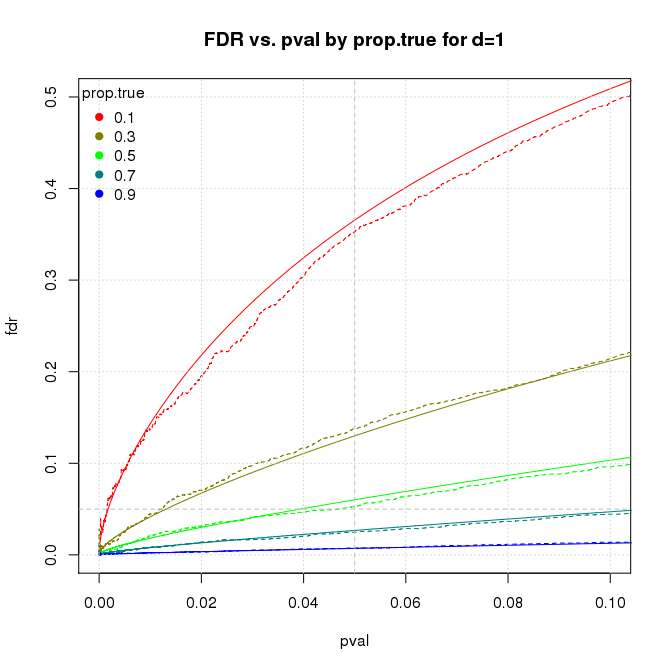
\includegraphics[width=0.5\linewidth]{../figure/swfdr_base/plot_byprop}
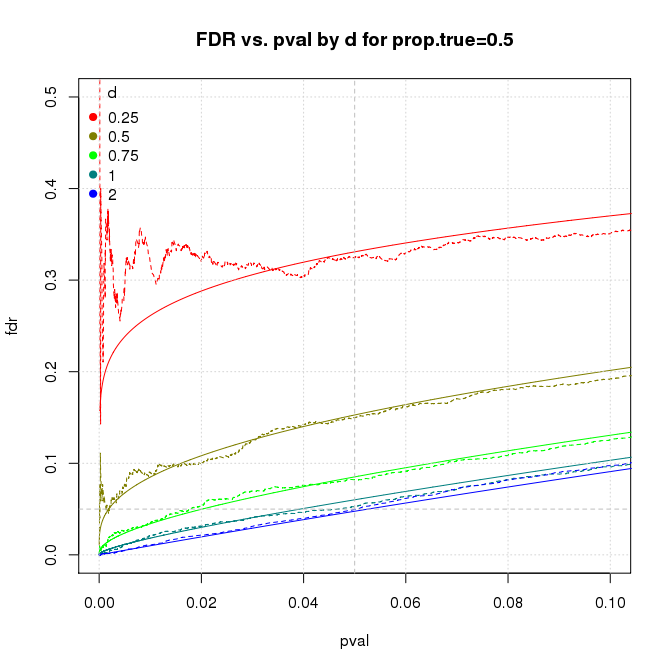
\includegraphics[width=0.5\linewidth]{../figure/swfdr_base/plot_byd}
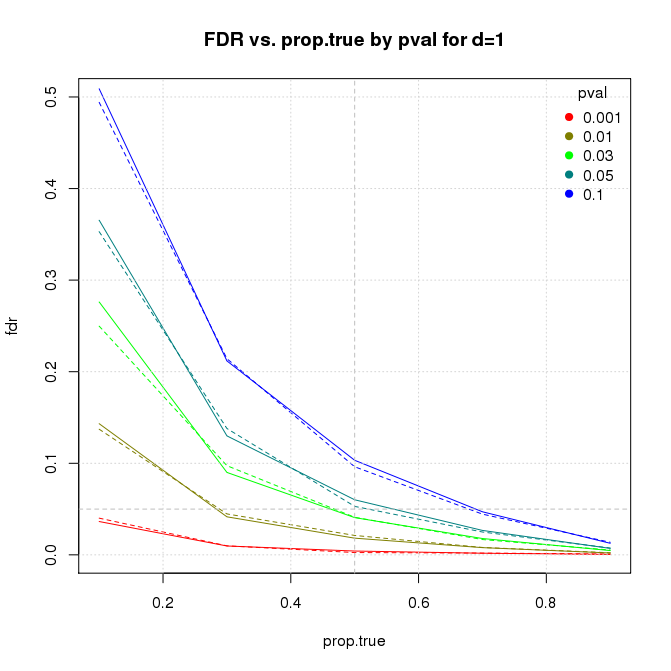
\includegraphics[width=0.5\linewidth]{../figure/swfdr_base/plot_vsprop}
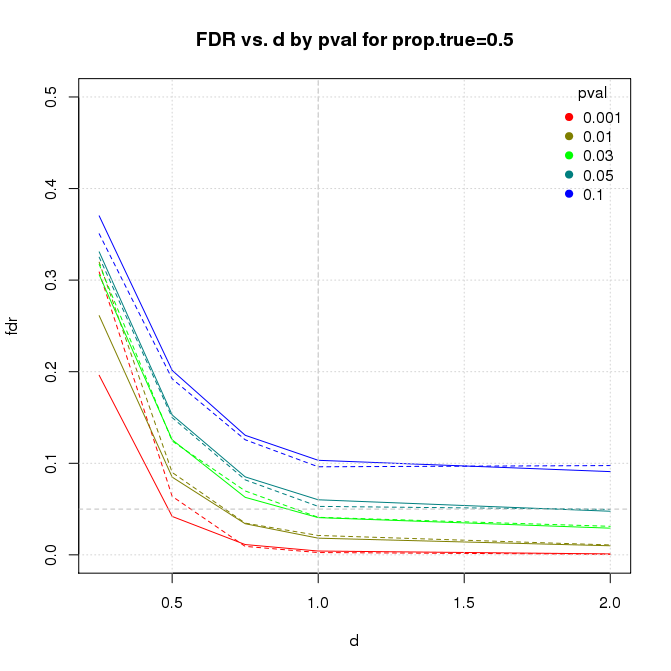
\includegraphics[width=0.5\linewidth]{../figure/swfdr_base/plot_vsd}

The notation is

\begin{itemize}
\tightlist
\item
  solid lines show theoretical results; dashed lines are empirical
  results from the simulation
\item
  \emph{fdr}. false discovery rate
\item
  \emph{pval}. p-value cutoff for significance
\item
  \emph{prop.true}. proportion of simulated cases that have a real
  effect
\item
  \emph{d}. standardized effect size, aka \emph{Cohen's d}
\end{itemize}

The user can change simulation parameters and control program operation
by providing new values to \texttt{run()} as illustrated in the example
code block above. The available parameters are

\begin{longtable}[]{@{}lll@{}}
\toprule
\begin{minipage}[b]{0.18\columnwidth}\raggedright\strut
parameter\strut
\end{minipage} & \begin{minipage}[b]{0.56\columnwidth}\raggedright\strut
meaning\strut
\end{minipage} & \begin{minipage}[b]{0.18\columnwidth}\raggedright\strut
default\strut
\end{minipage}\tabularnewline
\midrule
\endhead
\begin{minipage}[t]{0.18\columnwidth}\raggedright\strut
prop.true\strut
\end{minipage} & \begin{minipage}[t]{0.56\columnwidth}\raggedright\strut
fraction of cases where there is a real effect\strut
\end{minipage} & \begin{minipage}[t]{0.18\columnwidth}\raggedright\strut
\texttt{seq(.1,.9,by=.2)}\strut
\end{minipage}\tabularnewline
\begin{minipage}[t]{0.18\columnwidth}\raggedright\strut
m\strut
\end{minipage} & \begin{minipage}[t]{0.56\columnwidth}\raggedright\strut
number of iterations\strut
\end{minipage} & \begin{minipage}[t]{0.18\columnwidth}\raggedright\strut
\texttt{1e4}\strut
\end{minipage}\tabularnewline
\begin{minipage}[t]{0.18\columnwidth}\raggedright\strut
n\strut
\end{minipage} & \begin{minipage}[t]{0.56\columnwidth}\raggedright\strut
sample size\strut
\end{minipage} & \begin{minipage}[t]{0.18\columnwidth}\raggedright\strut
\texttt{16}\strut
\end{minipage}\tabularnewline
\begin{minipage}[t]{0.18\columnwidth}\raggedright\strut
d\strut
\end{minipage} & \begin{minipage}[t]{0.56\columnwidth}\raggedright\strut
standardized effect size (aka \emph{Cohen's d})\strut
\end{minipage} & \begin{minipage}[t]{0.18\columnwidth}\raggedright\strut
\texttt{c(.25,.50,.75,1,2)}\strut
\end{minipage}\tabularnewline
\begin{minipage}[t]{0.18\columnwidth}\raggedright\strut
pwr\strut
\end{minipage} & \begin{minipage}[t]{0.56\columnwidth}\raggedright\strut
power. if set, program adjusts \emph{d} to achieve power\strut
\end{minipage} & \begin{minipage}[t]{0.18\columnwidth}\raggedright\strut
\texttt{NA}\strut
\end{minipage}\tabularnewline
\begin{minipage}[t]{0.18\columnwidth}\raggedright\strut
sig.level\strut
\end{minipage} & \begin{minipage}[t]{0.56\columnwidth}\raggedright\strut
significance level for power calculations when \emph{pwr} is set\strut
\end{minipage} & \begin{minipage}[t]{0.18\columnwidth}\raggedright\strut
\texttt{0.05}\strut
\end{minipage}\tabularnewline
\begin{minipage}[t]{0.18\columnwidth}\raggedright\strut
pval.plot\strut
\end{minipage} & \begin{minipage}[t]{0.56\columnwidth}\raggedright\strut
p-values for which we plot results\strut
\end{minipage} & \begin{minipage}[t]{0.18\columnwidth}\raggedright\strut
\texttt{c(.001,.01,.03,.05,.1)}\strut
\end{minipage}\tabularnewline
\begin{minipage}[t]{0.18\columnwidth}\raggedright\strut
\strut
\end{minipage} & \begin{minipage}[t]{0.56\columnwidth}\raggedright\strut
\strut
\end{minipage} & \begin{minipage}[t]{0.18\columnwidth}\raggedright\strut
\strut
\end{minipage}\tabularnewline
\begin{minipage}[t]{0.18\columnwidth}\raggedright\strut
scriptname\strut
\end{minipage} & \begin{minipage}[t]{0.56\columnwidth}\raggedright\strut
used to set output directories and in error messages\strut
\end{minipage} & \begin{minipage}[t]{0.18\columnwidth}\raggedright\strut
\texttt{\textquotesingle{}swfdr\_base\textquotesingle{}}\strut
\end{minipage}\tabularnewline
\begin{minipage}[t]{0.18\columnwidth}\raggedright\strut
datadir\strut
\end{minipage} & \begin{minipage}[t]{0.56\columnwidth}\raggedright\strut
data directory relative to distribution root\strut
\end{minipage} & \begin{minipage}[t]{0.18\columnwidth}\raggedright\strut
\texttt{\textquotesingle{}data/swfdr\_base\textquotesingle{}}\strut
\end{minipage}\tabularnewline
\begin{minipage}[t]{0.18\columnwidth}\raggedright\strut
figdir\strut
\end{minipage} & \begin{minipage}[t]{0.56\columnwidth}\raggedright\strut
figure directory relative to distribution root\strut
\end{minipage} & \begin{minipage}[t]{0.18\columnwidth}\raggedright\strut
\texttt{\textquotesingle{}figure/swfdr\_base\textquotesingle{}}\strut
\end{minipage}\tabularnewline
\begin{minipage}[t]{0.18\columnwidth}\raggedright\strut
save\strut
\end{minipage} & \begin{minipage}[t]{0.56\columnwidth}\raggedright\strut
save parameters, results, and plots; sets \emph{save.rdata} and
\emph{save.plot}, not \emph{save.txt}\strut
\end{minipage} & \begin{minipage}[t]{0.18\columnwidth}\raggedright\strut
\texttt{FALSE}\strut
\end{minipage}\tabularnewline
\begin{minipage}[t]{0.18\columnwidth}\raggedright\strut
save.rdata\strut
\end{minipage} & \begin{minipage}[t]{0.56\columnwidth}\raggedright\strut
save parameters and results in RData format\strut
\end{minipage} & \begin{minipage}[t]{0.18\columnwidth}\raggedright\strut
\texttt{FALSE} (set by \emph{save})\strut
\end{minipage}\tabularnewline
\begin{minipage}[t]{0.18\columnwidth}\raggedright\strut
save.txt\strut
\end{minipage} & \begin{minipage}[t]{0.56\columnwidth}\raggedright\strut
save results in txt format. \textbf{CAUTION: big and slow}\strut
\end{minipage} & \begin{minipage}[t]{0.18\columnwidth}\raggedright\strut
\texttt{FALSE} (not set by \emph{save})\strut
\end{minipage}\tabularnewline
\begin{minipage}[t]{0.18\columnwidth}\raggedright\strut
save.plot\strut
\end{minipage} & \begin{minipage}[t]{0.56\columnwidth}\raggedright\strut
save plots\strut
\end{minipage} & \begin{minipage}[t]{0.18\columnwidth}\raggedright\strut
\texttt{FALSE} (set by \emph{save})\strut
\end{minipage}\tabularnewline
\begin{minipage}[t]{0.18\columnwidth}\raggedright\strut
clean\strut
\end{minipage} & \begin{minipage}[t]{0.56\columnwidth}\raggedright\strut
remove contents of data and figure directories; sets \emph{clean.data}
and \emph{clean.fig}\strut
\end{minipage} & \begin{minipage}[t]{0.18\columnwidth}\raggedright\strut
\texttt{FALSE}\strut
\end{minipage}\tabularnewline
\begin{minipage}[t]{0.18\columnwidth}\raggedright\strut
clean.data\strut
\end{minipage} & \begin{minipage}[t]{0.56\columnwidth}\raggedright\strut
remove contents of data directory\strut
\end{minipage} & \begin{minipage}[t]{0.18\columnwidth}\raggedright\strut
\texttt{FALSE} (set by \emph{clean})\strut
\end{minipage}\tabularnewline
\begin{minipage}[t]{0.18\columnwidth}\raggedright\strut
clean.fig\strut
\end{minipage} & \begin{minipage}[t]{0.56\columnwidth}\raggedright\strut
remove contents of figure directory\strut
\end{minipage} & \begin{minipage}[t]{0.18\columnwidth}\raggedright\strut
\texttt{FALSE} (set by \emph{clean})\strut
\end{minipage}\tabularnewline
\bottomrule
\end{longtable}

\subsubsection{Statistical Details}\label{statistical-details}

\begin{itemize}
\tightlist
\item
  The program assumes normally distributed data with equal variance.
\item
  The p-values are from a two-sided, unpaired, equal variance t-test
  (R's \texttt{t.test} with default settings for \texttt{alternative},
  \texttt{paired}, and \texttt{var.equal}).
\item
  The default sample size (\(n=16\)) gives about 80\% power for \(d=1\)
  and \(sig.level=0.05\). Power for the full range of \(d\) is
\end{itemize}

\begin{longtable}[]{@{}lllllc@{}}
\toprule
\emph{d} & 0.25 & 0.50 & 0.75 & 1.00 & 2.00\tabularnewline
\midrule
\endhead
power & 0.10 & 0.28 & 0.54 & 0.78 & 0.9998\tabularnewline
\bottomrule
\end{longtable}

\subsection{Directory Structure}\label{directory-structure}

The root directory contains the usual GitHub files: LICENSE, README.md,
.gitignore. There's also a NEWS.md file that lists major differences
between releases. The subdirectories are

\begin{itemize}
\tightlist
\item
  \texttt{css/} - style sheets used by the document generation process
\item
  \texttt{data/} - data files
\item
  \texttt{doc/} - documentation
\item
  \texttt{figure/} - plots
\item
  \texttt{script/} - scripts
\item
  \texttt{tool/} - helper scripts for the document generation process
\end{itemize}

\subsection{Other Scripts}\label{other-scripts}

TBD

\subsection{Functions}\label{functions}

\subsubsection{\texorpdfstring{\texttt{run} - \emph{Run the
program.}}{run - Run the program.}}\label{run---run-the-program.}

\paragraph{Description}\label{description}

Top-level function. Sets parameters (via \texttt{init}), does the work
(via \texttt{doit}) and optionally saves the results (via
\texttt{saveit})

\paragraph{Usage}\label{usage}

\begin{Shaded}
\begin{Highlighting}[]
\NormalTok{run=function(...)}
\end{Highlighting}
\end{Shaded}

\paragraph{Arguments}\label{arguments}

\begingroup
\setlength{\tabcolsep}{10pt} \renewcommand{\arraystretch}{1.2}
\centering

\begin{tabular}{m{\dimexpr0.15\columnwidth-\columnsep}m{\dimexpr0.50\columnwidth-\columnsep}m{\dimexpr0.25\columnwidth-\columnsep}}
\toprule
argument & meaning & default\\
\midrule
\texttt{...} & parameters passed to \texttt{init} & see \texttt{init} \\
\bottomrule
\end{tabular}

\endgroup

\paragraph{Value}\label{value}

This function is invoked for its side-effect. It has no return value.

\paragraph{Examples}\label{examples}

\begin{Shaded}
\begin{Highlighting}[]
\CommentTok{# this code block assumes your working directory is the root of the repository}

\KeywordTok{source}\NormalTok{(}\StringTok{"script/swfdr_base.R"}\NormalTok{);}
\CommentTok{# run default process}
\KeywordTok{run}\NormalTok{();}

\CommentTok{# run default process and save results in directories data/guide01 and figure/guide01}
\KeywordTok{run}\NormalTok{(}\DataTypeTok{save=}\NormalTok{T,}\DataTypeTok{datadir=}\StringTok{'data/guide01'}\NormalTok{,}\DataTypeTok{figdir=}\StringTok{'figure/guide01'}\NormalTok{);}

\CommentTok{# reduce runtime by reducing number of simulation runs and simulated cases}
\KeywordTok{run}\NormalTok{(}\DataTypeTok{m=}\FloatTok{1e3}\NormalTok{,}\DataTypeTok{d=}\KeywordTok{c}\NormalTok{(}\FloatTok{0.25}\NormalTok{,}\FloatTok{0.5}\NormalTok{,}\DecValTok{1}\NormalTok{),}\DataTypeTok{prop.true=}\KeywordTok{c}\NormalTok{(}\FloatTok{0.3}\NormalTok{,}\FloatTok{0.5}\NormalTok{,}\FloatTok{0.8}\NormalTok{));}

\CommentTok{# specify power directly and let program adjust effect size}
\KeywordTok{run}\NormalTok{(}\DataTypeTok{m=}\FloatTok{1e3}\NormalTok{,}\DataTypeTok{pwr=}\KeywordTok{c}\NormalTok{(}\FloatTok{0.1}\NormalTok{,}\FloatTok{0.3}\NormalTok{,}\FloatTok{0.8}\NormalTok{),}\DataTypeTok{prop.true=}\KeywordTok{c}\NormalTok{(}\FloatTok{0.3}\NormalTok{,}\FloatTok{0.5}\NormalTok{,}\FloatTok{0.8}\NormalTok{));}
\end{Highlighting}
\end{Shaded}

\paragraph{See Also}\label{see-also}

\protect\hyperlink{init}{\texttt{init}} for more information.

\subsubsection{\texorpdfstring{\texttt{init} - \emph{Initialize program
parameters.}}{init - Initialize program parameters.}}\label{init---initialize-program-parameters.}

\paragraph{Description}\label{description-1}

Processes parameters and stores them in global variables. Creates
parameter grid, called \texttt{cases}, containing all combinations of
parameters. Creates output directories if they do not exist.

\paragraph{Usage}\label{usage-1}

\begin{Shaded}
\begin{Highlighting}[]
\KeywordTok{init}\NormalTok{(}\DataTypeTok{prop.true =} \KeywordTok{seq}\NormalTok{(}\FloatTok{0.1}\NormalTok{, }\FloatTok{0.9}\NormalTok{, }\DataTypeTok{by =} \FloatTok{0.2}\NormalTok{),}
     \DataTypeTok{m =} \DecValTok{10000}\NormalTok{,}
     \DataTypeTok{n =} \DecValTok{16}\NormalTok{,}
     \DataTypeTok{d =} \KeywordTok{c}\NormalTok{(}\FloatTok{0.25}\NormalTok{, }\FloatTok{0.5}\NormalTok{, }\FloatTok{0.75}\NormalTok{, }\DecValTok{1}\NormalTok{, }\DecValTok{2}\NormalTok{),}
     \DataTypeTok{pwr =} \OtherTok{NA}\NormalTok{, }\DataTypeTok{sig.level =} \FloatTok{0.05}\NormalTok{,}
     \DataTypeTok{pval.plot =} \KeywordTok{c}\NormalTok{(}\FloatTok{0.001}\NormalTok{, }\FloatTok{0.01}\NormalTok{, }\FloatTok{0.03}\NormalTok{, }\FloatTok{0.05}\NormalTok{, }\FloatTok{0.1}\NormalTok{),}
     \DataTypeTok{scriptname =} \StringTok{"swfdr_base"}\NormalTok{,}
     \DataTypeTok{datadir =} \KeywordTok{file.path}\NormalTok{(}\StringTok{"data"}\NormalTok{, scriptname),}
     \DataTypeTok{figdir =} \KeywordTok{file.path}\NormalTok{(}\StringTok{"figure"}\NormalTok{, scriptname),}
     \DataTypeTok{save =} \NormalTok{F, }\DataTypeTok{save.rdata =} \NormalTok{save, }\DataTypeTok{save.txt =} \NormalTok{F, }\DataTypeTok{save.plot =} \NormalTok{save,}
     \DataTypeTok{clean =} \NormalTok{F, }\DataTypeTok{clean.data =} \NormalTok{clean, }\DataTypeTok{clean.fig =} \NormalTok{clean)}
\end{Highlighting}
\end{Shaded}

\paragraph{Arguments}\label{arguments-1}

\begingroup
\setlength{\tabcolsep}{10pt} \renewcommand{\arraystretch}{1.2}
\centering

\begin{tabular}{m{\dimexpr0.15\columnwidth-\columnsep}m{\dimexpr0.50\columnwidth-\columnsep}m{\dimexpr0.25\columnwidth-\columnsep}}
\toprule
argument & meaning & default\\
\midrule
\texttt{prop.true} & fraction of cases where where there is a real effect. & \texttt{seq(0.1, 0.9, by = 0.2)} \\
\texttt{m} & number of iterations. & \texttt{1e4} \\
\texttt{n} & sample size. & \texttt{16} \\
\texttt{d} & standardized effect size (aka \textit{Cohen's d}) & \texttt{c(0.25, 0.5, 0.75, 1, 2)} \\
\texttt{pwr} & power. if set, program adjusts \texttt{d} to achieve power. & \texttt{NA} \\
\texttt{sig.level} & significance level for power calculation & \texttt{0.05} \\
\texttt{pval.plot} & p-values for which we plot results & \texttt{c(1e-03, 0.01, 0.03, 0.05, 0.1)} \\
\texttt{scriptname} & script name. Used to construct output directory path names. & \texttt{"swfdr\_base"} \\
\texttt{datadir} & path name of directory for data files. & \texttt{"data/swfdr\_base"} \\
\texttt{figdir} & path name of directory for plots. & \texttt{"figure/swfdr\_base"} \\
\texttt{save} & logical. sets \texttt{save.rdata} and \texttt{save.plot} & \texttt{FALSE} \\
\texttt{save.rdata} & if TRUE, save parameters and results (actually, all global variables) in RData format. The output filename is \texttt{globals.RData} in directory \texttt{datadir}. & \texttt{FALSE} (set by \texttt{save}) \\
\texttt{save.txt} & save simulation and interpolation results as tab-delimited text files. The output filenames are \texttt{sim.txt} amd \texttt{interp.txt} in directory \texttt{datadir}. \textbf{CAUTION: big \& slow!} & \texttt{FALSE} \\
\texttt{save.plot} & if TRUE, save plots as png files in \texttt{figdir}. The output filenames are \texttt{plot\_byd.png}, \texttt{plot\_byprop.png}, \texttt{plot\_vsd.png}, \texttt{plot\_vsprop.png} & \texttt{FALSE} (set by \texttt{save}) \\
\texttt{clean} & logical. sets \texttt{clean.data} and \texttt{clean.fig}. & \texttt{FALSE} \\
\texttt{clean.data} & if TRUE, delete contents of datadir and start fresh & \texttt{FALSE} (set by \texttt{clean}) \\
\texttt{clean.fig} & if TRUE, delete contents of figdir and start fresh & \texttt{FALSE} (set by \texttt{clean}) \\
\bottomrule
\end{tabular}

\endgroup

\paragraph{Value}\label{value-1}

The \texttt{cases} data frame is returned invisibly.

\paragraph{Details}\label{details}

For the default parameters, the \texttt{cases} parameter grid expands to
25 cases (5 values of prop.true x 5 values of d; all other parameters
have single-valued defaults). We do 10,000 simulations for each case for
a total of 250,000 simulations. This takes about 3 minutes on my small
Linux server.

This function is usually called by \texttt{run}. It may be called
directly if the user wishes to perform custom initialization.

\paragraph{Examples}\label{examples-1}

\begin{Shaded}
\begin{Highlighting}[]
\CommentTok{# initialize parameters with default values}
\KeywordTok{init}\NormalTok{();}

\CommentTok{# initialize parameters with default values but save results in directories data/guide01 and plots in figure/guide01}
\KeywordTok{init}\NormalTok{(}\DataTypeTok{save=}\NormalTok{T,}\DataTypeTok{datadir=}\StringTok{'data/guide01'}\NormalTok{,}\DataTypeTok{figdir=}\StringTok{'figure/guide01'}\NormalTok{);}

\CommentTok{# initialize parameters with values requiring less runtime by reducing number of simulation runs and simulated cases}
\KeywordTok{init}\NormalTok{(}\DataTypeTok{m=}\FloatTok{1e3}\NormalTok{,}\DataTypeTok{d=}\KeywordTok{c}\NormalTok{(}\FloatTok{0.25}\NormalTok{,}\FloatTok{0.5}\NormalTok{,}\DecValTok{1}\NormalTok{),}\DataTypeTok{prop.true=}\KeywordTok{c}\NormalTok{(}\FloatTok{0.3}\NormalTok{,}\FloatTok{0.5}\NormalTok{,}\FloatTok{0.8}\NormalTok{));}

\CommentTok{# specify power directly and let program adjust effect size}
\KeywordTok{init}\NormalTok{(}\DataTypeTok{m=}\FloatTok{1e3}\NormalTok{,}\DataTypeTok{pwr=}\KeywordTok{c}\NormalTok{(}\FloatTok{0.1}\NormalTok{,}\FloatTok{0.3}\NormalTok{,}\FloatTok{0.8}\NormalTok{),}\DataTypeTok{prop.true=}\KeywordTok{c}\NormalTok{(}\FloatTok{0.3}\NormalTok{,}\FloatTok{0.5}\NormalTok{,}\FloatTok{0.8}\NormalTok{));}
\end{Highlighting}
\end{Shaded}

\subsubsection{\texorpdfstring{\texttt{doit} - \emph{Do the
work.}}{doit - Do the work.}}\label{doit---do-the-work.}

\paragraph{Description}\label{description-2}

Runs simulation (via \texttt{dosim}), interpolates relevant columns of
the simulation results at fixed p-values (via \texttt{dointerp}), and
plots the results and optionally save the plots (via \texttt{doplot}).

\paragraph{Usage}\label{usage-2}

\begin{Shaded}
\begin{Highlighting}[]
\NormalTok{doit=function()}
\end{Highlighting}
\end{Shaded}

\paragraph{Value}\label{value-2}

This function is invoked for its side-effect. It has no return value.

\protect\hypertarget{doplot}{}{}\protect\hypertarget{plot_byprop}{}{}\protect\hypertarget{plot_byd}{}{}\protect\hypertarget{plot_vsprop}{}{}\protect\hypertarget{plot_vsd}{}{}

\subsubsection{\texorpdfstring{Plot Functions - \emph{Plot the
results}}{Plot Functions - Plot the results}}\label{plot-functions---plot-the-results}

\paragraph{Description}\label{description-3}

These functions operate on the \texttt{sim} and \texttt{interp} data
frames produced by \texttt{dosim} and \texttt{dointerp} respectively.

\paragraph{Usage}\label{usage-3}

\begin{Shaded}
\begin{Highlighting}[]
\NormalTok{doplot=function(}\DataTypeTok{save.plot=}\NormalTok{F)}

\NormalTok{plot_byprop=function(}\DataTypeTok{save.plot=}\NormalTok{F,}\DataTypeTok{d1=}\DecValTok{1}\NormalTok{,}\DataTypeTok{sig.level=}\NormalTok{.}\DecValTok{05}\NormalTok{)}

\NormalTok{plot_byd=function(}\DataTypeTok{save.plot=}\NormalTok{F,}\DataTypeTok{prop.true1=}\FloatTok{0.5}\NormalTok{,}\DataTypeTok{sig.level=}\NormalTok{.}\DecValTok{05}\NormalTok{)}

\NormalTok{plot_vsprop=function(}\DataTypeTok{save.plot=}\NormalTok{F,}\DataTypeTok{d1=}\DecValTok{1}\NormalTok{,}\DataTypeTok{sig.level=}\NormalTok{.}\DecValTok{05}\NormalTok{)}

\NormalTok{plot_vsd=function(}\DataTypeTok{save.plot=}\NormalTok{F,}\DataTypeTok{prop.true1=}\FloatTok{0.5}\NormalTok{,}\DataTypeTok{sig.level=}\NormalTok{.}\DecValTok{05}\NormalTok{)}
\end{Highlighting}
\end{Shaded}

\paragraph{Arguments}\label{arguments-2}

\begingroup
\setlength{\tabcolsep}{10pt} \renewcommand{\arraystretch}{1.2}
\centering

\begin{tabular}{m{\dimexpr0.15\columnwidth-\columnsep}m{\dimexpr0.50\columnwidth-\columnsep}m{\dimexpr0.25\columnwidth-\columnsep}}
\toprule
argument & meaning & default\\
\midrule
\texttt{save.plot} & if TRUE, save the plot. The output format is PNG. The output filename is the name of the function with \texttt{.png} suffix  in directory \texttt{figdir}, eg, \texttt{figure/plot\_byprop.png}. & \texttt{FALSE} \\
\texttt{d1} & fixed value of \texttt{d} for dimension reduction. If \texttt{d1} is not in the \texttt{d} vector, it is set d1 to \texttt{max(d)}. & \texttt{1} \\
\texttt{prop.true1} & fixed value of \texttt{prop.true} for dimension reduction. If \texttt{prop.true} is not in the \texttt{prop.true} vector, it is set to the first value in \texttt{prop.true}. & \texttt{0.5} \\
\texttt{sig.level} & values of p-value and FDR marked by dashed lines on the plot. & \texttt{0.05} \\
\bottomrule
\end{tabular}

\endgroup

\paragraph{Details}\label{details-1}

\texttt{doplot} is the main plot function. It calls separate functions
for each of the four kinds of plot. * \texttt{plot\_byprop} plots FDR by
prop.true for one value of d * \texttt{plot\_byd} plots FDR by d for one
value of prop.true * \texttt{plot\_vsprop} plots FDR vs prop.true for
one value of d at fixed p-values * \texttt{plot\_vsd} plots FDR vs d for
one value of prop.true at fixed p-values

Each of the \texttt{plot\_} functions plots a different slice of
theoretical and empirical FDR as a function of three variables:
FDR=f(prop.true,d,pval) The functions differ in how they reduce four
dimensions (FDR and the three variables) to something that can be
plotted in two dimensions.

Each function starts by fixing one variable to a single value. Next, the
function splits the data into groups based on a second variable.
Finally, it plots each group vs.~the remaining variable, using different
line types (solid vs dashed) to distinguish theoretical and empirical
FDR.

\texttt{plot\_byprop} and \texttt{plot\_byd} operate on \texttt{sim};
\texttt{plot\_vsprop} and \texttt{plot\_vsd} operate on \texttt{interp}.

\subsection{Documentation}\label{documentation}

The documentation comprises

\begin{itemize}
\tightlist
\item
  this User Guide
\item
  \href{README.pdf}{README}
\item
  \href{NEWS.pdf}{NEWS} lists major differences between releases
\item
  R-style \href{TBD}{function-level documentation}
\item
  \href{science.pdf}{Science: Science-Wise False Discovery Rate}
  explains the scientific concepts underlying the software
\item
  \href{software.pdf}{Software: Science-Wise False Discovery Rate}
  discusses the software design and design choices
\item
  \href{exercises.pdf}{Exercises: Science-Wise False Discovery Rate}
  provides exercises for the reader to improve the program
\end{itemize}

Document files have several formats.

\begin{enumerate}
\def\labelenumi{\arabic{enumi}.}
\tightlist
\item
  R markdown (\texttt{Rmd}) is the source format. I generate the ooutput
  formats programmatically using, e.g.,
\end{enumerate}

\begin{Shaded}
\begin{Highlighting}[]
\NormalTok{rmarkdown::}\KeywordTok{render}\NormalTok{(doc/README.Rmd,}\StringTok{'github_document'}\NormalTok{)}
\NormalTok{rmarkdown::}\KeywordTok{render}\NormalTok{(doc/guide.Rmd,(}\KeywordTok{c}\NormalTok{(}\StringTok{'html_document'}\NormalTok{,}\StringTok{'pdf_document'}\NormalTok{))}
\end{Highlighting}
\end{Shaded}

\begin{enumerate}
\def\labelenumi{\arabic{enumi}.}
\setcounter{enumi}{1}
\tightlist
\item
  markdown (\texttt{md}) is the output format GitHub prefers for
  documents displayed on its site. Due to limitations in GitHub's
  \texttt{md} support, I only use this format for simple documents,
  viz,. README and NEWS.
\item
  \texttt{html}. These are self-contained HTML files that should display
  correctly on your local computer or website. Because they are
  self-contained, they tend to be huge and inscrutable. Note that GitHub
  shows HTML files as raw text, which is not very illuminating, but has
  an \href{http://htmlpreview.github.io}{HTML preview feature} that
  renders the files as expected.
\item
  \texttt{pdf}. GitHub renders the files as expected \textbf{but
  disables links}.
\end{enumerate}

\subsection{See Also}\label{see-also-1}

Felix Schönbrodt's
\href{http://www.nicebread.de/whats-the-probability-that-a-significant-p-value-indicates-a-true-effect/}{blog
post} and \href{http://shinyapps.org/apps/PPV/}{ShinyApp} got me going
down this path and offer an insightful, different perspective. Blog
posts by
\href{http://daniellakens.blogspot.de/2015/09/how-can-p-005-lead-to-wrong-conclusions.html}{Daniel
Lakens} and
\href{http://willgervais.com/blog/2014/9/24/power-consequences\%3E}{Will
Gervais} are also interesting.

Papers by
\href{http://rsos.royalsocietypublishing.org/content/1/3/140216}{David
Colquhoun}, \href{http://doi.org/10.1093/biostatistics/kxt007}{Leah
Jager and Jeffrey Leek}, and
\href{http://dx.plos.org/10.1371/journal.pmed.0020124}{John Ioannidis}
cover it all with full statistical rigor and much more detail.

\subsection{Author}\label{author}

Nathan (Nat) Goodman, (natg at shore.net)

\subsection{Bugs and Caveats}\label{bugs-and-caveats}

Please report any bugs, other problems, and feature requests using the
\href{https://github.com/natgoodman/FDR/issues}{GitHub Issue Tracker}. I
will be notified, and you'll be apprised of progress.

\subsubsection{Known Bugs and Caveats}\label{known-bugs-and-caveats}

\begin{itemize}
\tightlist
\item
  The simulation results are noisy for \(m\) \textless{} 5x103 and
  dubious for \(m\) \textless{} 103; the program does not run at all for
  \(m\) \textless{} 2.
\item
  The software is pretty basic. See \href{exercises.pdf}{Exercises:
  Science-Wise False Discovery Rate} for a list of known limitations.
\end{itemize}

\subsection{Copyright \& License}\label{copyright-license}

Copyright (c) 2017 Nathan Goodman

The software is \textbf{open source and free}, released under the
\href{https://opensource.org/licenses/MIT}{MIT License}.


\end{document}
